\documentclass[letterpaper, 11pt]{article}
%\usepackage{palatino}%
\usepackage{hyperref}
\usepackage{graphicx}
\usepackage{caption}
\usepackage{subcaption}
\renewcommand{\baselinestretch}{1.1}
\usepackage[margin=1.2in]{geometry}
\usepackage{xcolor}
\hypersetup{
    colorlinks,
    linkcolor={red!50!black},
    citecolor={blue!50!black},
    urlcolor={blue!80!black}
}

\begin{document}
\title{WebPlotDigitizer User Manual\\ Version 3.9}
\author{Ankit Rohatgi\footnote{E-Mail: ankitrohatgi@hotmail.com}}
\maketitle
\tableofcontents
\newpage
\section{Introduction}
A large quantity of technical data is available only in the form of plots and images. In these images, it is easy to visualize the relationship between the variables involved, but recovering the exact numerical values of the data is usually a tedious and error prone process. To aid this time consuming task of data recovery, many digitization tools have been developed over the years, but this task remains daunting and prone to errors. The common complains with the existing tools are as follows:

\begin{itemize}
\item{Limited in features, often supporting only a few specific plot types.}
\item{Compatible with only some specific operating systems.}
\item{Difficult to use or prone to errors.}
\item{No longer maintained by the original developer.}
\item{Closed source or no freedom to modify the code.}
\end{itemize}

Because of the above limitations with the current digitizing tools, WebPlotDigitizer was developed to facilitate easy and accurate data extraction from a variety of plot types. This program has been built using HTML5 which allows it to run within most popular web browsers and does not require to be installed by the user. This is distributed free of charge as an opensource software and since its creation in 2011, this tool has gained thousands of users and has been cited in many published articles. A screenshot of a typical session of the software is shown in Figure \ref{fig:screenshot}.

\begin{figure}
\begin{center}
\fbox{\includegraphics[width=6in]{./figures/screenshot.png}}
\caption{Screenshot of WebPlotDigitizer showing the data points recovered on a plot via automatic detection.}
\label{fig:screenshot}
\end{center}
\end{figure}

\subsection{History}
WebPlotDigitizer was initially developed while working on my graduate studies at the University of Notre Dame. Having to extract data from many publications for comparing and contrasting my own findings in the lab was a time consuming task. The search for a tool to aid this process usually ended in realizing that most of the existing tools for this purpose did not fulfill many of the requirements. 

Some of the experimental work in the lab required me to learn some basic image processing techniques which eventually formed the basis of the automatic detection algorithms used here. Image processing knowledge along with some interest in learning the very popular HTML5 APIs were a perfect match to create a web based data extraction tool like this.

WebPlotDigitizer is now used by thousands everyday and because of this interest, I have continued to maintain and improve the software in my spare time.

\subsection{User Manual and Tutorials}
This user manual describes the various capabilities of the software and aims to help the user in making an effective use of the software. This manual may be updated continuously to match the latest deployed version of the software. A few video tutorials for the previous version of the software are available at \url{http://arohatgi.info/WebPlotDigitizer}. If the you want me to document the underlying theory and algorithms, then please write me an email.

\subsection{License}
WebPlotDigitizer is distributed under GNU General Public License version 3 by Ankit Rohatgi. For the complete terms and conditions, please refer to \url{http://www.gnu.org/copyleft/gpl.html}

\subsection{Source Code}
WebPlotDigitizer is an open source software (see above). The source code can be obtained from GitHub (\url{https://github.com/ankitrohatgi/WebPlotDigitizer/}). Feel free to contact via email if you wish to contribute to this project.

\subsection{Availability}
The latest stable version of the software can be used directly from the website \url{http://arohatgi.info/WebPlotDigitizer}. For the Google Chrome web browser, an \emph{app} pointing to the online software is also available at the Chrome App Store (\url{https://chrome.google.com/webstore/category/apps}).

\subsection{Supported Browsers}
The HTML5 capabilities required by WebPlotDigitizer have been available in all popular browsers for the last 2 to 3 years. Version 3.9 was ensured to work without any issues on recent versions of Google Chrome, Firefox, Safari, Internet Explorer and Microsoft Edge.


\subsection{Citing WebPlotDigitizer}
If you wish to cite WebPlotDigitizer in any of your works, then please use the following information:

\begin{center}
\begin{tabular}{|r|l|}
\hline
Author & Ankit Rohatgi\\
Title & WebPlotDigitizer\\
Website & \url{http://arohatgi.info/WebPlotDigitizer}\\
Version & 3.9\\
Date & August, 2015\\
E-Mail & ankitrohatgi@hotmail.com\\
Location & Austin, Texas, USA\\
\hline
\end{tabular}
\end{center}

\subsection{Reporting Issues}
Feel free to contact via e-mail to report issues or offer suggestions. If you are comfortable with GitHub, then please use the issue tracker for this project: \url{https://github.com/ankitrohatgi/WebPlotDigitizer/issues}

\subsection{Data Privacy}
WebPlotDigitizer's image analysis code runs entirely on the user's computer and does not store the loaded images or data on to any server. When \emph{Graph in Plotly} option is selected, the digitized data is transmitted to Plotly (\url{http://plot.ly}) servers. For a detailed privacy policy, please refer to \url{http://arohatgi.info/WebPlotDigitizer/privacy.html}.

\subsection{Funding}
WebPlotDigitizer is not funded by any organization. This project is entirely supported by the PayPal donations from generous supporters and my personal time and effort.

\section{Loading Plots}
The image file containing the figure to be analyzed can be loaded into the software in the following ways:
\begin{enumerate}
\item{{\bf Drag \& Drop Operation:} Image can be dragged and dropped from the file browser on to the image viewing area of the application.}
\item{{\bf File Menu $\rightarrow$ Load Image:} Browse for a file on the hard disk to load.}
\item{{\bf Copy-Paste from Clipboard:} This is only supported in Google Chrome web browser. An image selected by copying in a PDF or an image viewer can be pasted on to the software via a simple copy-paste operation.}
\item{{\bf File Menu $\rightarrow$ Webcam Capture:} A snapshot taken from the webcam can also be used. For best results, the webcam should be pointed directly along the normal to the plot surface. In the future, some perspective transformation tools might be added to WebPlotDigitizer to compensate for the distortions when the camera is not perfectly aligned.}  
\end{enumerate}

\subsection{Supported Image Formats}
WebPlotDigitizer relies on the image formats supported by the HTML5 \emph{canvas} element. Most browsers support common image formats such as JPEG, PNG, BMP and GIF. Since the support for an image format depends on the browser used to access the software, please refer to your browser's manual for details. For popular browsers, you can also refer to Wikipedia (\url{http://en.wikipedia.org/wiki/Comparison_of_web_browsers#Image_format_support}).

Please note that loading PDF files directly is not supported. It is recommended that you use the tools built into your PDF reader to save the image of the region of interest or copy the image area into the clipboard and paste into WebPlotDigitizer. Pasting images from the clipboard is only supported for Google Chrome.


\section{Calibrate Axes}

After loading the desired image, you should specify the type of axes that is used in the plot. This step is required for the software to correctly map the image pixels to the corresponding data values in the image. Depending on the plot type, you will have to select a few known points on the axes. On clicking the \emph{Axes $\rightarrow$ Calibrate Axes} menu item, you should be presented with the menu shown in Figure \ref{fig:defineAxesPopup}.
\begin{figure}
\begin{center}
\fbox{\includegraphics[width=3in]{./figures/defineAxesPopup.png}}
\caption{Popup with plot types that are supported in the software.}
\label{fig:defineAxesPopup}
\end{center}
\end{figure}

\subsection{2D (X-Y) Plot}
Most plots that are on a two dimensional cartesian coordinate system fall under this category. Plots with non-orthogonal axes or plots rotated by an angle should work just fine, but images with perspective distortions will not yield accurate results. You can use image editing tools such as Gimp (\url{http://www.gimp.org/}) to correct the perspective distortions before using WebPlotDigitizer.

After selecting the 2D (X-Y) plot option, another popup window appears with instructions to click on two points on the horizontal axis and two points on the vertical axis. After reading these instructions, and closing this popup, click on two points on one of the axes $(x_1, x_2)$ and two on the other $(y_1, y_2)$. For better accuracy during the digitization process, pick the points that are as far away from each other as possible. Note down the data values at $(x_1, x_2)$ and $(y_1, y_2)$ positions as you will be required to enter those once the four points have been clicked on.

During selection of the four points, you can also make fine adjustments to the location of a calibration point that is highlighted in green using keyboard cursor keys. Pressing the \emph{Shift}-key along with the cursor keys will move the point at a faster rate. To highlight a different point than what is already selected, you just need to click on the other point after the four points have been placed on the screen. Zooming into the image can help improve the accuracy.

After the four points have been clicked on, press \emph{Continue} and another popup window will appear where you will be required to enter the values at these points. This helps the software map the image pixels corresponding to data points to their actual values when the image is digitized. To view the mapping equations, select the \emph{Transformation Equations} option from the \emph{Axes} menu.

\begin{figure}
\centering
{\begin{subfigure}[b]{0.4\textwidth}
\includegraphics[width=\textwidth]{./figures/xyAxesInfo.png}
\caption{Mark four points to align axes}
\end{subfigure}
\begin{subfigure}[b]{0.4\textwidth}
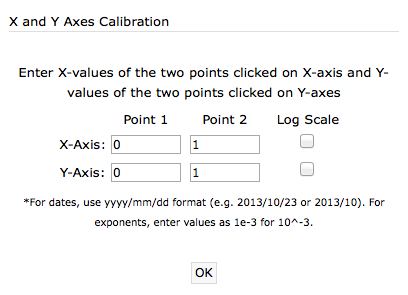
\includegraphics[width=\textwidth]{./figures/xyAlignment.png}
\caption{Specify values}
\end{subfigure}}
\caption{Alignment for 2D (X-Y) Plot.}
\label{fig:xyAlignment}
\end{figure}

\subsubsection{Calibration Value Format}
\label{sec:formattingInput}
Like most computer programs, WebPlotDigitizer accepts integers (e.g. 1, 2, 3 etc.) or floating point numbers (e.g. 3.14159). Some extra things to keep in mind are as follows:
\begin{enumerate}
\item{Fractions are not computed as numbers. Entering $1/2$ (for example), will not be considered as 0.5.}
\item{For exponentials, the caret symbol (\^{}) is not recognized and the values have to be entered as 1.45e-10 for $1.45 \times 10^{-10}$ (for example).}
\item{{\bf Dates:} This is enabled only for 2D (X-Y) Plots. At the time of calibration, the dates have to be entered in the format shown below. With the final digitized data, however, results can be formatted in many different ways (see section \ref{sec:formattingDatesCSV}).
\begin{center}
\begin{tabular}{|c|c|c|}
\hline
Date & Format & Examples\\
\hline
Year, Month and Date & YYYY/MM/DD & 2012/10/23, 2012/10/5 or 2012/10/05\\
Year, Month & YYYY/MM & 2012/10 or 1989/5\\
Year & YYYY & 2012 (treated as any integer)\\
\hline
\end{tabular}
\end{center}
}
\end{enumerate}


\subsection{Bar Charts}

\subsubsection{Bar Charts vs. Histograms}
For bar charts with a continuous variation of data along the data axis, but with only a discrete set of labels on the other, select the \emph{2D Bar Plot} option when calibrating the axes. For plots such as histograms where both the axes are continuously varying, you should still select the \emph{2D (X-Y) Plot} option and use the manual mode or the \emph{histogram} algorithm for data extraction.

\subsubsection{Axes Calibration for Bar Charts}
Select the \emph{2D Bar Plot} option when calibrating the axes and follow the instructions to select two points on the continuously varying data axis that is along the bars. Next, specify the values at these two points so that WebPlotDigitizer can construct a mathematical relationship between the pixel position along this axis and the corresponding data value.

After calibration, you can manually click on the bars to mark the points or use the automatic extraction mode where you can use the color of the bars to extract data points. For bar charts, you can also edit the labels of each individual data point.

\subsection{Polar Diagram}
Select this option if the data points in the image are plotted on a polar axes. On selecting this, you will be required to click on three known points including the center of the polar diagram (Figure \ref{fig:polarAlignment}). After clicking on 3 points, you can also select the axes orientation and select Degrees or Radians for the angle. For log-polar diagrams, you can select the log scale option. The values entered here also have to follow the format similar to 2D (X-Y) Plots. Dates can not be used for values in this case.

\begin{figure}
\centering
{\begin{subfigure}[b]{0.4\textwidth}
\includegraphics[width=\textwidth]{./figures/polarInfo.png}
\caption{Mark three points to align axes}
\end{subfigure}
\begin{subfigure}[b]{0.3\textwidth}
\includegraphics[width=\textwidth]{./figures/polarAlignment.png}
\caption{Specify values}
\end{subfigure}}
\caption{Alignment for Polar Diagram.}
\label{fig:polarAlignment}
\end{figure}
 
\subsection{Ternary Diagram}
Ternary phase diagrams are harder to interpret than simple two dimensional cartesian or polar plots. Using this software to recover data makes the process of data recovery extremely straightforward and thus reduces the possibility of misinterpreting the data. For this type of plot, simply mark the three corners as shown in the instructions and then specify the range of variables and orientation of the diagram (Figure \ref{fig:ternaryAlignment}).

\begin{figure}
\centering
{\begin{subfigure}[b]{0.4\textwidth}
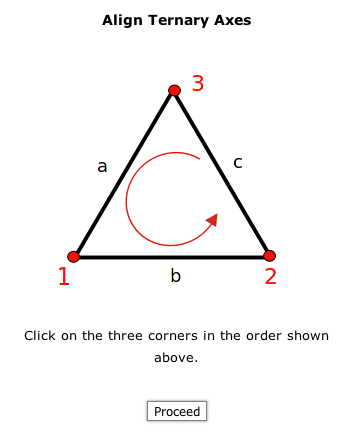
\includegraphics[width=\textwidth]{./figures/ternaryInfo.png}
\caption{Mark three points to align axes}
\end{subfigure}
\begin{subfigure}[b]{0.4\textwidth}
\includegraphics[width=\textwidth]{./figures/ternaryAlignment.png}
\caption{Specify values}
\end{subfigure}}
\caption{Alignment for Ternary Diagram.}
\label{fig:ternaryAlignment}
\end{figure}

\subsection{Maps/Microscope Images}
The \emph{Map with Scale Bar} option is similar to 2D (X-Y) Plots and is to be used for images that only have scale information (e.g. microscope images or maps). To calibrate the pixels to the scale bar in these images, simply click on the two ends of the scale bar and enter the scale value. You can also specify the label to be used for the unit (Figure \ref{fig:mapAlignment}). The coordinates reported by the software assume the origin to be located at the top left of the image with positive y-axes pointing downwards. The (x,y) values that are generated are scaled using the value entered during calibration.

\begin{figure}
\centering
{\begin{subfigure}[b]{0.3\textwidth}
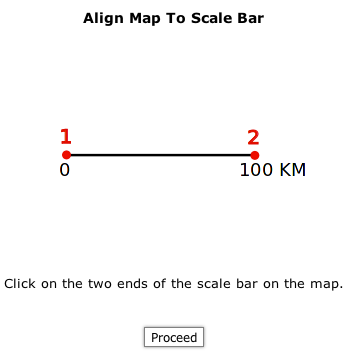
\includegraphics[width=\textwidth]{./figures/mapInfo.png}
\caption{Mark ends of the scale bar}
\end{subfigure}
\begin{subfigure}[b]{0.3\textwidth}
\includegraphics[width=\textwidth]{./figures/mapAlignment.png}
\caption{Specify the scale value and the unit label}
\end{subfigure}}
\caption{Alignment for maps and microscope images.}
\label{fig:mapAlignment}
\end{figure}

\subsection{Image (Align to Image Pixels)}
This plot type is similar to the Map plot type and is provided just as a convenience to work with generic images. If you select this type, no calibration information is required as the software will just do a 1:1 mapping from the image pixels to data values. This plot type is useful when the exact pixel locations of the image features are required.

\subsection{Transformation Equations}
After calibrating the axes, you can select the \emph{Transformation Equations} option in the \emph{Axes} menu to view the relationship that is constructed by WebPlotDigitizer to convert image pixels to data. This feature allows users to use this mapping in other graphics codes or softwares where it may be required to convert image pixel locations to corresponding data or vice versa.

\section{Grid Removal}
The automatic extraction algorithms of WebPlotDigitizer rely on the color differences between the data points or curves and the background. This approach works only when there are very few background artifacts of the same color as the data. In many plots with grid lines, it is difficult for the extraction algorithms to distinguish between the background grid lines and the data curves (often in the same color). For such plots, a grid removal tool has been added, that can be used to remove the interfering horizontal and vertical lines present in the image before data extraction.

\section{Acquire Data}

Once the plot axes have been calibrated, you can begin selecting data points on the image. Also note that the numbers below the zoom window reflect actual data coordinates corresponding to your mouse position on the image. If you see incorrect numbers here, then perhaps incorrect calibration values were entered. You must repeat the axes calibration in this situation. 

WebPlotDigitizer should also show a side panel with the data acquisition controls (Figure \ref{fig:acquireData}) when the axes are aligned. This sidebar can also be brought up by selecting the \emph{Acquire Data} option in the \emph{Data} menu. The data acquisition can be performed in either manual or automatic mode. You can alternate between the two modes at any time. In the manual mode you can add, adjust or remove data points by manually clicking at the desired locations. In the automatic mode, you can set up and execute an extraction algorithm that can differentiate between the data points and the image background and identify several data points in a short time.

\begin{figure}
\centering
{
\begin{subfigure}{0.3\textwidth}
\includegraphics[width=\textwidth]{./figures/manualSidebar.png}
\caption{Manual Mode}
\end{subfigure}
\begin{subfigure}{0.3\textwidth}
\includegraphics[width=\textwidth]{./figures/autoSidebar.png}
\caption{Automatic Mode}
\end{subfigure}
}
\caption{Data acquisition controls.}
\label{fig:acquireData}
\end{figure}

\subsection{Manual Mode}
The controls available in this mode are as follows:
\begin{enumerate}
\item{{\bf Dataset: }Pick the dataset from the list to specify the data series the data points are to be added to (or modified). See section \ref{sec:multipleDatasets} for further details.}
\item{{\bf Automatic Mode: }Switch to automatic extraction mode.}
\item{{\bf Add Point (A): }After clicking this button or pressing the 'A' key, you can click in the image area to add data points. Any point added on the image will automatically be converted from on-screen pixels to data values utilizing the axes calibration.}
\item{{\bf Adjust Point (S): }After clicking this or pressing the 'S' key, you can click on an existing data point to select it. The selected point can then be repositioned using the cursor keys on the keyboard. Press Shift+Cursor key for a faster rate of movement.}
\item{{\bf Delete Point (D): }After clicking this button or pressing the 'D' key, you can click on a previously added data point to delete it.}
\item{{\bf Clear Points: }This deletes all data points added on the image. This does not clear the axes calibration.}
\item{{\bf View Data: }This launches a popup dialog where the collected data can be viewed, exported to a CSV file or Plotly. See section \ref{sec:csvData} for details.}
\item{{\bf Edit Labels: }This option is only available for Bar Charts.}
\end{enumerate}

\subsection{Automatic Mode}
The controls available in the automatic mode are used for selecting the appropriate algorithm and providing the necessary inputs required for automated extraction of data points. 

Automatic data extraction relies on separating the color of the data points or curves from the background in the image. The extraction algorithms can work in two modes of color extraction: Foreground mode and Background mode. In the foreground mode, the algorithms look for the foreground color specified for the data and ignore everything else. In the background mode, the algorithms include everything except the background color as potential data points. If the data points or curves of interest are uniformly colored (approximately), then the foreground mode may be more suitable. Otherwise if the background is uniformly colored (approximately) and the curve or data points are not then the background mode may me more suitable.

The extraction algorithms also need to know the region of the image to be searched for the specified colors. The software does not search the entire image as in many cases, the data point or the curve colors may be repeated in non-data parts of the image. To specify the region of interest, use the \emph{Box}, \emph{Pen} and \emph{Erase} tools (described below) to paint over a yellow mask over the data part of the image as shown in Figure \ref{fig:markRegion}. The extraction algorithms will look for data only under  the yellow colored region. The various controls available in this mode are as follows:
\begin{figure}
\begin{center}
\includegraphics[width=4in]{./figures/markRegion.png}
\caption{Use the \emph{Box}, \emph{Pen} and \emph{Erase} tools to mark the region containing the required data (automatic extraction).}
\label{fig:markRegion}
\end{center}
\end{figure}




\begin{enumerate}
\item{{\bf Dataset: }Pick the dataset from the list to specify the data series the data points are to be added to (or modified). See section \ref{sec:multipleDatasets} for further details.}
\item{{\bf Manual Mode: }Switch to manual mode. You can switch between these modes at any time.}
\item{{\bf Mask Controls:} These controls are to be used to mark the search region for the extraction algorithms. Use the following drawing tools to highlight the approximate region containing data. You should try to exclude all features that are similar in color to the desired data points.}
\begin{enumerate}
    \item{{\bf Box: }This is used to mark a rectangular region to be used during the search for data points.}
    \item{{\bf Pen: }This is used for marking areas of the image to be included in the search for data points via free hand drawing.}
    \item{{\bf Erase: }This is used to unmark the areas marked using the \emph{Box} or \emph{Pen} tools.}
    \item{{\bf View: }This is used to simply view the marked search region.}
\end{enumerate}
\item{{\bf Color Controls: } Use these controls to specify the color of the data points and an approximate RGB distance from this color that is acceptable. You either need to specify the foreground color of the data or the color of the background. In most cases, the distance value will require some hit-and-trial based on the results generated by the extraction algorithm.}
\begin{enumerate}
    \item{{\bf Foreground/Background Color Selection: }Select the appropriate option from the drop-down menu and click on the colored button on the right to show a popup for color selection. The popup dialog also shows a list of most dominant colors at the bottom that can be selected.}
    \item{{\bf Distance: }Change this value to adjust the range of colors around the selected color to be accepted as foreground or background.}
    \item{{\bf Filter Colors: }Test the color selection and the specified distance value. The area highlighted in yellow is the region that will finally be used by the automatic extraction algorithms.}
\end{enumerate}
\item{{\bf Algorithm Selection: }Select the appropriate algorithm depending on the application. Each algorithm is described in detail the next section.}
\item{{\bf Run: }Start the auto-detection algorithm. After this is completed, the detected points should appear over the image. If necessary, adjust the parameters of the extraction algorithm, mask or color settings and run the algorithm until you are satisfied. You can also switch to manual mode and edit these data points.}
\item{{\bf Clear All: }Clear all data points in the current dataset.}
\item{{\bf View Data: }This launches a popup dialog where the data can be viewed and exported to a CSV file or Plotly. See section \ref{sec:csvData} for details.}
\end{enumerate}

\subsection{Digitization Algorithms}
Four different digitization algorithms are available in WebPlotDigitizer as shown in Figure \ref{fig:autoExtractAlgos}. The \emph{Averaging Window} algorithm is set as the default as it is usually suitable in most simple cases.
\begin{figure}
\begin{center}
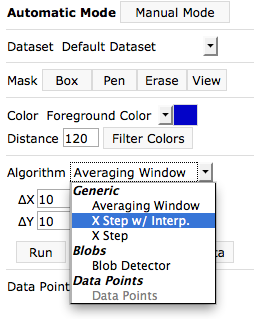
\includegraphics[width=2in]{./figures/wpd_algos.png}
\caption{Four automatic extraction algorithms are available. These are subject to change in the future releases.}
\label{fig:autoExtractAlgos}
\end{center}
\end{figure}
\subsubsection{Averaging Window}
As mentioned above, this is probably the most useful algorithm and is useful across many plot types. The data points detected by this algorithm are determined by calculating the average locations of pixels with acceptable color that lie in small regions that are $\Delta X$ pixels (on-screen) wide and $\Delta Y$ pixels (on-screen) tall. As a user, you should increase the size of this window for thick lines or large data points and decrease it for thin lines. If you see multiple points incorrectly detected across the width of a thick data curve, then you need to increase the numbers specified here. The fact that this requires on-screen pixels may be changed in the future so that the values in actual units in the current axes can be specified.

\subsubsection{X Step with Interpolation}
This algorithm is available only for non log-scale 2D (X-Y) axes plots. In the future, this will be extended to other axes types. This algorithm can identify data points at regular intervals on the X-axis that fall between $X_{min}$ and $X_{max}$ and $Y_{min}$ and $Y_{max}$. The data points are spaced at an interval $\Delta X$ units apart. This algorithm interpolates over missing data using cubic splines and is therefore suitable even for curves with dotted lines or a series with just data points. The \emph{Smoothing} value can be increased from zero (for example, try 0.5) to average over a larger neighborhood around the data points. This is useful for reducing noise in the captured data. (Also see: \url{http://arohatgi.info/WebPlotDigitizer/blog/posts/discontinuous_data.html})

\subsubsection{X Step}
This is a simplified version of the \emph{X Step with Interpolation} algorithm. This does not use cubic splines to interpolate over data. The \emph{Line Width} parameter is the y-direction thickness of the curve in on-screen pixels (In future, this will be updated to use the appropriate units in Y). 

\subsubsection{Blob Detector}
This algorithm is useful for counting number of objects, determining the location of their centroids, calculating areas and also first moments of continuous objects. All objects that are within the \emph{Min Diameter} and \emph{Max Diameter} range are added as data points. (Also see: \url{http://arohatgi.info/WebPlotDigitizer/blog/posts/blob_detection.html})

\subsubsection{Bar Charts and Histograms}

\section{Multiple Datasets}
\label{sec:multipleDatasets}
For plots that have multiple sets of data, you can capture data for one dataset, export the CSV file, then clear all the data points and start over to collect data for the next set. This may be acceptable in many cases, but this is can be somewhat inconvenient if you wish to return to an old dataset and modify some data points. Also, this way, you will not be able to store data for all the datasets in an exported JSON file (see section \ref{sec:csvData}). 

A better option is to create a separate dataset for each series you wish to capture by selecting the \emph{Add} option in the \emph{Manage Dataset} popup that can be accessed from the \emph{Data} menu (Figure \ref{fig:manageDatasets}). From this popup, you can also delete or rename a dataset. After adding multiple sets, you can then switch between these from the dataset menus available in the manual and automatic extraction controls and also in the \emph{View Data} window. By default, one dataset called "Default Dataset" is available.
\begin{figure}
\begin{center}
\includegraphics[width=3.5in]{./figures/wpd_dataset_2.png}
\caption{Add, delete or rename datasets corresponding to each series of data in the plot.}
\label{fig:manageDatasets}
\end{center}
\end{figure}

 
\section{Handling Digitized Data}
\label{sec:csvData}
Once the required data points are marked on the image using the manual mode, automatic mode or a combination of both, the digitized values can be seen by clicking the \emph{View Data} button. This presents a popup window as shown in Figure \ref{fig:csvOutput}. Here, the digitized values can be sorted by the variable or in order of the distance between the points (Nearest Neighbor). The values can also be copied and used in common data analysis softwares. Recently, an option to send these values over to another cloud based data analysis and graphing software called Plotly (\url{http://plot.ly}) has also been added.
 
\begin{figure}
\begin{center}
\includegraphics[width=6in]{./figures/wpd_formatting.png}
\caption{CSV formatted digitized data. This can be sorted, pasted to a .CSV file or graphed in Plotly.}
\label{fig:csvOutput}
\end{center}
\end{figure}
\subsection{Sort Data}
The digitized data can be left unsorted (Raw Output) or by one of the axes variables in ascending or descending order. The Nearest Neighbor option sorts the data depending on the distance of the points from each other.
\subsection{Formatting Dates}
\label{sec:formattingDatesCSV}
If one or both of the axes in a 2D (X-Y) plot contain dates then fields to specify the output format of the values are also shown (Figure \ref{fig:dateFormat}). In these fields, the following pieces of text are replaced with the corresponding part of the date to format the text (case insensitive):
\begin{figure}
\begin{center}
\includegraphics[width=2.5in]{./figures/dateFormat.png}
\caption{Field to specify formatting of dates. This appears on X, Y or both axes depending on which variables contained dates at the time of axes calibration.}
\label{fig:dateFormat}
\end{center}
\end{figure}


\begin{center}
\begin{tabular}{|c|c|c|}
\hline
Text & Replaced With & Example\\
\hline
YYYY or yyyy & Year, all digits & 2012\\
YY or yy & Year, last two digits & 98 for 1998\\
MMMM or mmmm & Month, full name & January\\
MMM or mmm & Month, short name & Jan\\
MM or mm & Month, numeric & 10\\
DD or dd & Date & 23\\
\hline
\end{tabular}
\end{center}

A few examples are shown below:

\begin{center}
\begin{tabular}{|c|c|}
\hline
Format Field Text & Date Shown (Example)\\
\hline
dd-mm-yyyy & 23-10-2012\\
mmm-yyyy & Oct-2012\\
yyyy abc mmmm & 2012 abc October\\
mmm 'yy & Oct '12\\
\hline
\end{tabular}
\end{center}

\subsection{Number Formatting}
The number formatting of the digitized data columns can be changed by specifying the number of digits and the formatting style from the menu. Three formatting styles are available at the moment: 
\begin{enumerate}
\item{{\bf Fixed:} Use this to display the desired number of digits after the decimal.}
\item{{\bf Precision:} Use this to set the number of significant digits.}
\item{{\bf Exponential: } Use scientific notation with the desired number of digits after the decimal.}
\end{enumerate}
The \emph{Ignore} option disables the number formatting.

\subsection{Export to .CSV File}
Comma-Separated Values (CSV) format files are simple text files containing tabular data. Each row of line corresponds to a table row and the column values are separated by a character or a string (usually just a comma)\footnote{For more information on CSV format, check out \url{http://en.wikipedia.org/wiki/Comma-separated_values}}. Due to its simplicity, CSV format is supported in most data analysis softwares like Microsoft Excel, Matlab etc.

To save the values from WebPlotDigitizer into a CSV file, all you have to do is open your favorite text editor (e.g. Notepad on Microsoft Windows) and Copy-Paste the values shown in the results popup window. Save the file with a .CSV file extension. You can now use this file in your favorite data analysis software.


\section{Distance and Angle Measurements}
Besides extracting data points from plots, WebPlotDigitizer can also be used to make some simple distance and angle measurements on images. In the future, many more advanced analysis tools will be added. To make distance or angle measurements, choose the appropriate option from the \emph{Analysis} menu.

For distance measurements, if the chosen plot type is a \emph{Map} axes, then the distance is converted to the units specified during calibration. Otherwise distance values are shown in pixels on the original image (not same as on-screen pixels!). Angle measurements are not dependent on any axes. In each case, you can make a single measurement after pressing the \emph{Add} button (or pressing 'A' key) and then clicking on the image. After the measurement is made, you can adjust the highlighted (green) point using the cursor keys on the keyboard (use Shift for faster movement). To change the highlighted point, click on the desired point. A measurement can be deleted after clicking the \emph{Delete} button or pressing the key 'D'. \emph{Clear All} will delete all measurement data in that mode. \emph{View Data} will show a popup with all measurements that can be exported to \emph{Plotly} or a \emph{CSV} file.

\section{Import and Export JSON}
\label{sec:jsonImportExport}
If you wish to save the axes calibration, data points in all the datasets and the measurements to a file for future use, then you can select the \emph{Export JSON} option in the \emph{File} menu. Note that this file does not contain the image and so you will also have to keep the plot image along with this JSON file. To use the information stored in the JSON file, simply use the \emph{Import JSON} option in the \emph{File} menu. The Export and Import feature can also be used to reuse axes calibrations across multiple plot images which are plotted on the same axes.

\section{Custom Scripts}
Users can also create custom scripts to automate some of the digitization tasks or add new functionality. Custom scripts have access to most of the WebPlotDigitizer's API. A few examples can be seen on \url{http://github.com/ankitrohatgi/WebPlotDigitizer-Examples}. If you need help with custom scripts, then send me an email.

\section{Personal Hosting}
You can host WebPlotDigitizer on a personal or corporate network with just a simple HTTP server with PHP support. All image processing and other calculations related to the digitization occurs on the client browser, so the server does not need any significant resources. The PHP backend is used simply to bounce back CSV and JSON files to get around the restrictions imposed by HTML5.


\end{document}
